\chapter{Application}
\section{La proposition}
\subsection{L'objectif}
\paragraph{}Le but de l'application qui va suivre est de comparer différents modèles à la fois NoSQL et relationnels dans le but de déterminer le plus adapté par rapport aux données géographiques des SIG. Différents tests seront réalisés afin de mettre en lumière les forces et faiblesses de chacun. Lequel est le plus simple à modéliser, lequel a les meilleures vitesses d'exécution, lequel facilite la représentation sont des questions qui pourront se poser.


\subsection{Le choix des modèles}
\paragraph{}Afin de répondre à la question générale, plusieurs SGBD et modèles seront utilisés. Le premier sera le document. Son principal avantage est celui d'unité de la structure, supprimant le besoin de réaliser des jointures et permettant une meilleure adaptation à la distribution. Ce modèle s'avère grandement utilisé dans les outils de cartographie actuels comme avec le \newacronym{GML}{GML}{Geography Markup Language} \acrshort{GML} et ses dérivés : le \newacronym{KML}{KML}{Keyhole Markup Language} \acrshort{KML} utilisé par Google Earth et le OSM XML utilisé par OpenStreetMap. La structure des grammaires, encadrées par l'\acrfull{OGC} permet une meilleure interopérabilité.
%Le premier modèle qui sera utilisé sera le modèle graphe. Sa structure avec des noeuds et des arcs s'avère l'une des plus adaptées dans le cadre par exemple de calculs de distances.
%PARAGRAPHE A MODIFIER

%\paragraph{}Par ailleurs, un autre modèle sera implémenté, ce 

\paragraph{}Afin de comparer les modèles NoSQL à des modèles plus traditionnels que sont les bases de données relationnels, une étude sera faite sur une base qui suit les principes de Codd avec relations et nuplets.

\subsection{Le jeu d'essai}
\paragraph{}Le jeu d'essai utilisé dans le cadre de ce mémoire correspond aux résultats des élections municipales de 2020, plus précisément de son premier tour. Les données sont issues des sources gouvernementales fournies par le Ministère de l'Intérieur sur \url{data.gouv.fr}.

\paragraph{}Le fichier initial comprenait 68 815 lignes de données qui représentaient chacune les résultats d'un bureau de vote dans toutes les communes des 103 départements français (Outre-mer compris). Cependant, au vue de la quantité trop importante de données, il a été choisi de prendre uniquement les résultats franciliens (d'Ile-de-France) qui limite donc les données à 7 326 bureaux de votes, répartis sur 1268 communes à travers 8 départements. 

\paragraph{}Parmi les données répertoriées dans le fichier, nous avons les informations sur le département et la commune avec pour chacun leur nom et leur code. Sont également présentes les données sur le bureau de code : son numéro, le nombre d'inscrits, le nombre de votants, d'abstention, du nuls ou de blancs avec différents pourcentages basés sur le nombre de votants ou d'inscrits. Après cela, il y a les données sur les listes avec un numéro, la nuance politique et les informations sur le candidat (nom, prénom et sexe). Aussi, selon si c'est une commmune avec candidature par liste ou candidat, le nom de la liste est renseigné ou non. Concernant les résultats, sur chaque ligne de bureau de vote et pour chaque liste ou candidat, il y a le nombre de voix et le pourcentage par rapport au nombre d'inscrits et de votants.

\paragraph{}Par rapport à ce fichier, il a également été choisi de faire un tri comme un certain nombre de données calculées sont présentes alors qu'elles peuvent être calculées par le SGBD.

%Le fichier comprend 68 815 lignes de données quants i présentent chacune les résultats de chaque bureau de vote dans toutes les communes dans tous les départements de France métropolitaine et d'Outre-mer. Parmi les informations présentées, nous avons :
%\begin{itemize}
    %\item les informations sur le département : le code et le nom
    %\item les informations sur la commune : la partie commune du code INSEE et le nom
   % \item le bureau de vote : son code, le nombre d'inscrits, de votants, d'abstention et leur pourcentage respectif ainsi que le nombre de bulletins nuls, blancs et exprimés et leur pourcentage par rapport au nombre de votants et d'inscrits
    %\item les informations sur les listes : un code, le nuance politique, le sexe, le nom et prénom de la tête de liste et le nom de la liste associée
    %\item les résultats de chaque liste : le nombre de voix obtenues et le pourcentage par rapport au nombre de votants et d'inscrits
%\end{itemize}

%\paragraph{}Cependant, après réflexions autour de la pertinence de certaines données, il a été choisi d'enlever les pourcentages car même si ils évitent de devoir effectuer des calculs, ils occupent un espace qui pourrait être libéré.
%couplées aux données territoriales pour faire correspondre communes, départements, régions

\subsection{Les outils utilisés}
\paragraph{}Plusieurs outils seront utilisés dans le cadre de la réalisation de cette application. Plusieurs SGBD seront utilisés :
\begin{itemize}
    \item MySQL comme base de données relationnelle
    \item BaseX pour les aspects document
    %\item OrientDB ou Neo4j pour les graphes
\end{itemize}

\section{L'utilisation d'un modèle relationnel}

\subsection{Modélisation et implémentation}
\paragraph{}Le \acrshort{MCD} ci-dessous correspond à la représentation la plus adaptée du jeu de données en y enlevant les données calculées. On peut y voir qu'un département est composé de plusieurs communes avec pour chacune des bureaux de vote, des candidats et listes. La relation bureau de vote-candidat permet d'obtenir le nombre de voix obtenu pour ce candidat dans ce bureau.


%Le modèle conceptuel de données ci-dessous correspond à la représentation la plus adaptée des données. A partir de ce dernier a été généré un script SQL permettant la création de la base de données.
%\paragraph{}Dans le \acrshort{MCD} ci-dessous, on peut y voir qu'un département est composé de plusieurs communes et dépendent de ce département. Il peut par exemple avoir plusieurs villes avec le même nom mais dans des départements différents. Pour chacune de ces villes, il y a des bureaux de votes et des candidats ou listes qui lui sont associés et ces derniers obtiennent des résultats aux élections.
%Il prend en compte un certain tri des données. En effet, de nombreuses données calculées, des pourcentages, étaient présents. Cependant, ces données occupent de l'espace inutilement sachant que ces calculs peuvent être effectués par le SGBD.
\begin{figure}[!htp]
  \centering
  \includegraphics[width=.9\textwidth]{./src_img/image_mcd.png}
  \caption{Modèle Conceptuel de données}
  \label{fig:mcd}
\end{figure}

\subsection{Le peuplement de la base}


\paragraph{}Avec le MCD, un script SQL a permis la création de la base de données puis, pour la compléter, un code similaire à ce pseudo-code a été utilisé :\newline
\begin{algorithm}[H]
\KwData{fichier CSV}
 \KwResult{Base de données remplie}
 initialisation fichier\;
 \While{toutes les lignes ne sont pas parcourues}{
 \If{departement non présent}{ajouter département dans la base}
  \If{commune non présente}{ ajouter commune dans la base}
 \If{bureau de vote non présent}{ ajouter bureau dans la base}
 \While{ligne de données non finie d'être parcourue}{
 \If{liste/candidat non présent}{ ajouter liste/candidat dans la base}
 ajouter résultat\;
 }
 }
 \caption{Algorithme de peuplement de la base}
\end{algorithm}
\paragraph{}Dans cet algorithme, pour chaque élément qu'on souhaite ajouter, une vérification est nécessaire afin d'éviter d'avoir des doublons de bureaux ou candidats dans la base.

\paragraph{}En partant des critères définis au début de l'état de l'art, nous allons donc évaluer cette base de données.
\begin{table}[h!]
    \centering
	\begin{tabular}{|p{5cm}|p{7cm}|} 
  	\hline
  	\textbf{Critère} & \textbf{Valeur} \\
  	\hline
  	2.1 : taille occupé & 5,87 Mo \\
  	\hline
  	2.2 : nombre d'objets & 64 873 \\
  	\hline
	\end{tabular}
    \caption{Table des critères concernant la base de données MySQL}
    \label{tab:critere-mysqlbase}
\end{table}
\subsection{L'interrogation d'un SGBD relationnel}
\paragraph{}Afin de vérifier des performances de la base de données, diverses requêtes vont être réalisées :
\subsubsection{Une requête de recherche}
\paragraph{}La première requête va lister les communes des Yvelines (78) comprenant un 'r' dans leur nom avec le nombre de votants respectifs, triés par ordre décroissant.
%\paragraph{}Cette première requête va rechercher la liste des communes et leurs nombres de votants par ordre décroissant pour celles situées dans les Yvelines (78) et comprenant un R dans leur nom.
\paragraph{}Cette requête retourne 162 villes parmi lesquelles Versailles et Saint-Germain-en-Laye. Elle a été réalisée en 5 ms et a manipulé 814 objets (villes et bureaux de vote).

\iffalse
\begin{figure}[!ht]
    \begin{verbatim}
SELECT nom_ville, SUM(nb_inscrits) as nb_insc 
FROM ville, bureau_vote 
WHERE ville.code_dep = bureau_vote.code_dep 
  AND ville.code_ville = bureau_vote.code_ville 
  AND nom_ville LIKE '%r%' AND ville.code_dep='78' 
GROUP BY nom_ville 
ORDER BY nb_insc desc;
\end{verbatim}
    \caption{Requête de recherche}
\end{figure}
\fi

\subsubsection{Une requête de calcul et regroupement}
\paragraph{}La deuxième requête est destinée à calculer pour chaque département francilien le nombre de communes ayant un vote par liste et le nombre de celles ayant un vote par poste. Voici donc le résultat qu'elle a permis d'obtenir :
\begin{figure}[!htp]
  \centering
  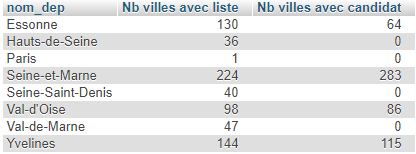
\includegraphics[width=0.6\textwidth]{./src_img/req2_sql.png}
  \caption{Données extraites de la 2ème requête}
  \label{fig:req2}
\end{figure}
\paragraph{}Cette requête, réalisée en 126 millisecondes en touchant à 12 574 objets, avait une petite spécificité. Habituellement, pour déterminer si l'élection est par liste ou candidat, on se base sur la population mais le jeu de données ne comporte pas cette donnée. Nous nous basons donc sur le champ du nom de la liste, vide si c'est une élection par candidat. %Habituellement, pour savoir si une ville a une élection par liste ou candidat, on se base sur la population de celle-ci. Hors, dans le jeu de données, nous n'avons que le nombre d'inscrits sur les listes électorales, excluant donc les mineurs. Pour savoir le type de l'élection, il a donc été choisi de vérifier si le champ du nom de liste parmi les listes et candidats présents étaient remplis ou non.
%\paragraph{}La deuxième requête est destinée à calculer pour chaque département francilien le nombre de communes ayant un vote par liste ou un vote par candidat. \newline Pour définir le type du vote, il est habituellement réalisé en fonction du nombre d'habitants de la commune. Or, ici, nous n'avons que le nombre d'inscrits sur les listes électorales, ce qui exclut donc les mineurs. Pour déterminer si le vote dans une commune se fait par liste ou candidat, nous nous sommes basés sur le nom de liste, vide si c'est une élection par candidat.
\iffalse
\begin{figure}[!ht]
    \begin{verbatim}
SELECT nom_dep, 
(SELECT count(distinct(nom_ville)) as nb from ville, liste
  where liste.code_dep=ville.code_dep and
  ville.code_ville=liste.code_ville  and
  liste.code_dep=dep.code_dep and 
  length(nom_liste)<>0) as `Nb villes avec liste`, 
(SELECT count(distinct(nom_ville)) as nb from ville, liste
  where liste.code_dep=ville.code_dep and
  ville.code_ville=liste.code_ville and
  liste.code_dep=dep.code_dep and 
  length(nom_liste)=0) as `Nb villes avec candidat`
FROM departement dep
GROUP BY nom_dep;
\end{verbatim}
    \caption{Requête de calcul et regroupement}
\end{figure}
\fi

%\paragraph{}Cette requête a été réalisée en 126 millisecondes.

%nombre moyen de listes par région

\subsubsection{Des taux en fonction de différents critères}
\paragraph{}Il a également choisi de vérifier les fonctions de calcul. Deux requêtes ont donc été réalisées dans ce but. La première liste les communes d'Ile-de-France triées suivant une absention décroissante. Elle a retournée 1268 résultats (soit toutes les communes franciliennes) en 4,96 ms tout en lisant 8 594 objets.
%- les régions/communes ayant enregistré le plus grand taux d'abstention

\iffalse
SELECT nom_ville, ville.code_dep,  ((SUM(nb_abstention)/SUM(nb_inscrits))*100) as taux FROM ville, bureau_vote WHERE ville.code_dep=bureau_vote.code_dep AND ville.code_ville=bureau_vote.code_ville GROUP BY nom_ville ORDER BY taux desc
\fi
%temps : 4,96 ms
\paragraph{}La deuxième requête retourne le taux de participation par département. Elle retourne donc 8 objets en 1,74 millisecondes tout en touchant à 8 602 objets.
%- taux de participation par région/commune
\iffalse
SELECT departement.nom_dep, SUM(nb_inscrits) as nbinsc, SUM(nb_votants) as nbvot, ((SUM(nb_votants)/SUM(nb_inscrits))*100) as taux
FROM departement, ville, bureau_vote WHERE departement.code_dep=ville.code_dep AND ville.code_dep=bureau_vote.code_dep AND ville.code_ville=bureau_vote.code_ville
GROUP BY departement.nom_dep
ORDER BY taux desc
\fi
%temps : 1,74 ms
\subsubsection{Une requête de mise à jour}
\paragraph{}La dernière requête est une mise à jour. Il a été choisi de modifier le nom d'une liste d'une commune. La requête a été réalisée en 0, 00044 ms en lisant qu'un seul objet.

%temps : 0,00044 ms
\subsubsection{Synthèse des résultats}
\paragraph{}La table \ref{tab:critere-req1mysqlbase} représente les résultats des critères définis auparavant. On peut y apercevoir une durée inférieure à 5 ms pour la plupart des requêtes mais également, en parallèle, un grand nombre d'objets manipulés.
\begin{table}[!h]
    \centering
	\begin{tabular}{|p{3cm}|p{3cm}|p{3cm}|p{3cm}|} 
  	\hline
  	\textbf{Requête} & \textbf{3.1 : temps} & \textbf{3.2 : nombre de résultats} & \textbf{3.3 : objets manipulés} \\

  	\hline
  	Requête 1 & 5 ms & 162 & 814 \\
  	\hline
    Requête 2 & 126 ms & 8 & 12 574 \\
    \hline
    Requête 3 & 4,96 ms & 1268 & 8 594 \\
    \hline
    Requête 4 & 1,74 ms & 8 & 8 602 \\
    \hline
    Requête 5 & 0,00044 ms & & 1 \\
    \hline
	\end{tabular}
    \caption{Table des critères concernant les requêtes via MySQL}
    \label{tab:critere-req1mysqlbase}
\end{table}
\newpage
\subsection{La représentation des données depuis MySQL}
\paragraph{}Après avoir pu comparer les résultats des requêtes, il peut être également intéressant de faire le tour des solutions possibles de représentation des données, MySQL ne permettant pas la visualisation graphique. Il existe deux catégories.

\subsubsection{Les logiciels de datavisualisation}
\paragraph{}Un grand nombre d'outils permettent de visualiser des données, répartis entre ceux uniquement dédiés à la visualisation et ceux permettant à l'aide à la décision via de la BI (Business Intelligence). Parmi ces outils, nous avons Tableau Software, Qlik Sense, Power BI et SAP Business Object BI. Ces outils permettent à la fois la représentation sous forme d'histogramme, de diagramme circulaire, de treemap voire même de cartes.
\subsubsection{Les librairies}
\paragraph{}En plus de ces logiciels, des librairies existent pour fonctionner avec diverses technologies pour les utiliser au sein de projets. Des langages orientés objet tels que Java, C\# peuvent les utiliser tout comme PHP, Ruby, Python ou JavaScript. Parmi ces librairies qui permettent la visualisation de graphiques, nous avons Chart.js, D3.js, Google Chart API ou Highcharts.

\paragraph{}La figure \ref{fig:graphMySQL} est par exemple le résultat de la requête concernant l'abstention par région. Ce diagramme a été réalisé grâce à Chart.js.

\begin{figure}[!htp]
  \centering
  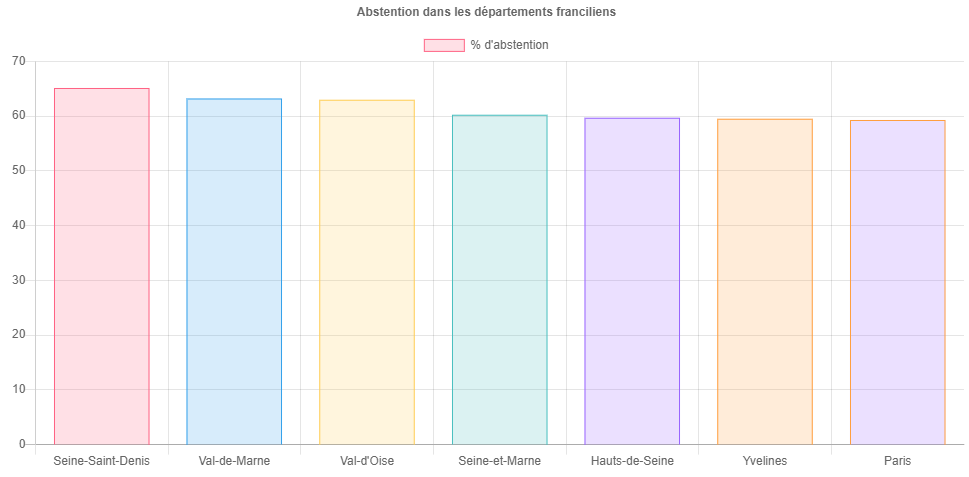
\includegraphics[width=0.6\textwidth]{./src_img/chartMySQLData.png}
  \caption{Graphique utilisant les données MYSQL}
  \label{fig:graphMySQL}
\end{figure}

%des requêtes, pour quoi ne chercher côté visualisation maintenant? 
%Est-ce que BaseX a des outils de visualisation intégrés?
%visualisation tableau des résultats des requêtes, mais de la visualisation graphique! Je ne connais pas BaseX pour te suggérer une piste, mais je pense qu'il est très intéressant de comparer  la possibilité d'affichage graphique des données relationnelles et données en documents (en brut ou résultat d'un requête).


\section{L'utilisation d'un modèle orienté document}

\subsection{Modélisation}
\paragraph{}La modélisation pour avoir un document s'est également basé sur une réflexion autour des données présentes. Celles présentes et répétées de nombreuses fois telles que les départements et communes ont été priorisées. Pour la gestion des bureaux et des listes, il a été choisi de proriser les bureaux de vote car ils correspondaient à la caractéristique principale de chaque ligne du jeu d'essai.

\begin{figure}[!htp]
  \centering
  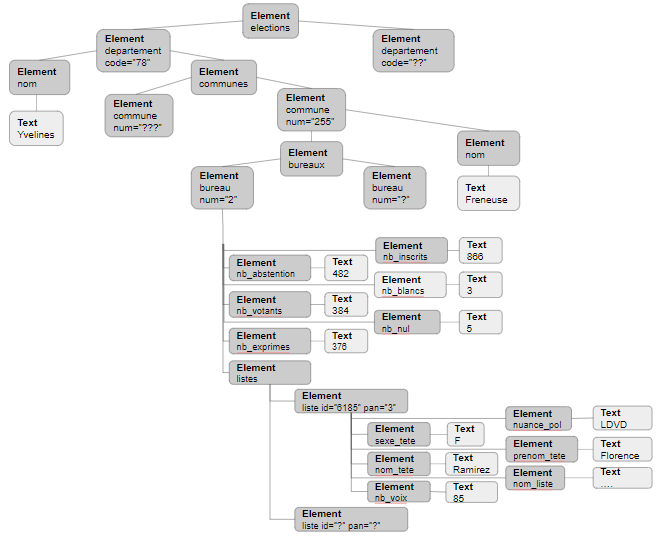
\includegraphics[width=\textwidth]{./src_img/structure_document.png}
  \caption{Modèle document}
  \label{fig:model_doc}
\end{figure}

\paragraph{}De la réflexion présentée est issue le modèle ci-dessus (figure \ref{fig:model_doc}) où nous avons à la base de la structure les départements dans lesquels sont ajoutés les communes qui le composent. Dans chacune de ces villes, nous retrouvons les différents bureaux de votes avec pour chacun les listes présentes, leurs informations et les résultats récoltés.
%\begin{figure}[!htb]
   %\begin{minipage}{0.48\textwidth}
    % \centering
     %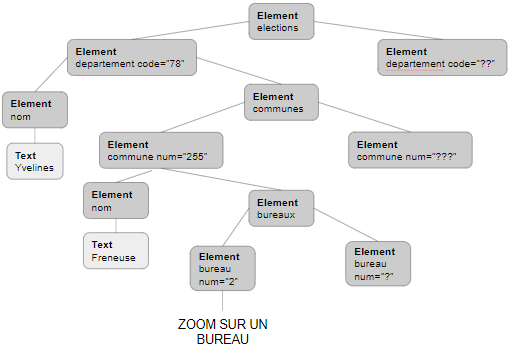
\includegraphics[width=\linewidth]{./src_img/modele_doc1.png}
     %\caption{Partie haute (département, ville et bureau)}\label{Fig:modele_doc1}
   %\end{minipage}\hfill
   %\begin{minipage}{0.48\textwidth}
   %  \centering
    % 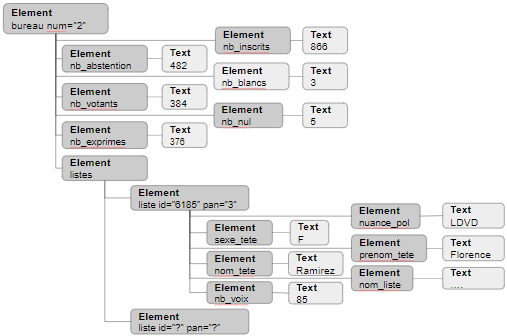
\includegraphics[width=\linewidth]{./src_img/modele_doc2.png}
    % \caption{Partie basse (détail d'un bureau et des listes et résultats)}\label{Fig:modele_doc2}
   %\end{minipage}
%\end{figure}

\subsection{L'implémentation du modèle avec les données}
\paragraph{}L'implémentation s'est faite à partir de ce modèle afin de donner un document XML apte à être utilisé. Par la suite, les données ont pu être insérées suivant l'algorithme suivant.

%a modifier
\begin{algorithm}[H]
 \KwData{fichier CSV}
 \KwResult{Base de données remplie}
 initialisation fichier\;
 \While{toutes les lignes ne sont pas parcourues}{
 \If{departement non présent}{ajouter département dans la base}
 déplacement dans le noeud du département\;
  \If{commune non présente}{ ajouter commune dans la base}
 déplacement dans le noeud de la commune\;
 \If{bureau de vote non présent}{ ajouter bureau dans la base}
 déplacement dans le noeud du bureau\;
 \While{tous les candidats/listes ne sont pas traités}{
 ajouter liste/candidat dans la base\;
 ajouter le résultat associé\;
 }
 }
 \caption{Algorithme de peuplement de la base}
\end{algorithm}

\paragraph{}En partant des critères définis au début de l'état de l'art, nous allons donc évaluer cette base de données.
\begin{table}[h!]
    \centering
	\begin{tabular}{|p{3cm}|p{9cm}|} 
  	\hline
  	\textbf{Critère} & \textbf{Valeur} \\
  	\hline
  	2.1 : taille & 10,58 Mo \\
  	\hline
  	2.2 : nombre d'objets & 673 942 noeuds parmi lesquels 53 575 correspondent aux départements, villes, bureaux et listes \\
  	\hline
	\end{tabular}
    \caption{Table des critères concernant la base de données XML}
    \label{tab:critere-xmlbase}
\end{table}
\paragraph{}Les résultats obtenus sont cohérents avec la structure du fichier XML, plus robuste qu'une base de données SQL.
\iffalse
\begin{figure}[!htb]
   \begin{minipage}{0.48\textwidth}
     \centering
     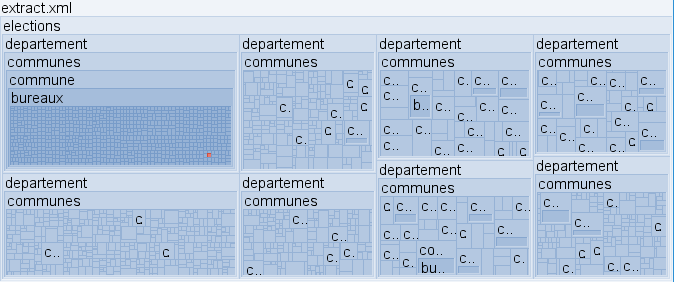
\includegraphics[width=.9\linewidth]{./src_img/modelisation_doc_1.png}
     \caption{Aperçu global}\label{Fig:doc_global}
   \end{minipage}\hfill
   \begin{minipage}{0.48\textwidth}
     \centering
     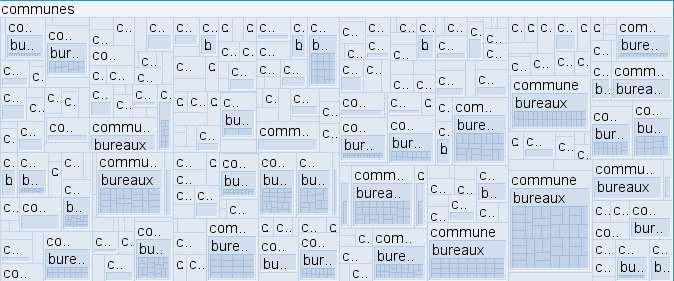
\includegraphics[width=.9\linewidth]{./src_img/modelisation_doc_2.png}
     \caption{Zoom sur les communes d'un département}\label{Fig:doc_dep}
   \end{minipage}
      \begin{minipage}{0.48\textwidth}
     \centering
     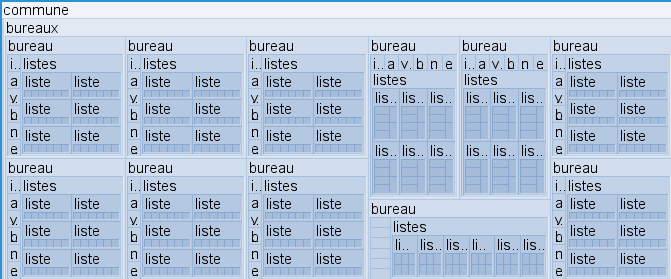
\includegraphics[width=.9\linewidth]{./src_img/modelisation_doc_3.png}
     \caption{Zoom sur une commune}\label{Fig:doc_commune}
   \end{minipage}\hfill
   \begin{minipage}{0.48\textwidth}
     \centering
     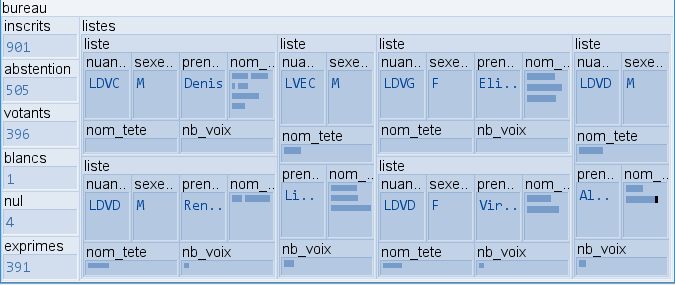
\includegraphics[width=.9\linewidth]{./src_img/modelisation_doc_4.png}
     \caption{Zoom sur un bureau}\label{Fig:doc_bureau}
   \end{minipage}
\end{figure}
\fi

\subsection{L'interrogation d'un SGBD document}


\paragraph{}Afin de vérifier des performances de la base de données, nous allons reprendre les mêmes besoins que pour le SGBD relationnel :

\subsubsection{Une requête de recherche}
\paragraph{}Nous reprenons la requête qui va lister les communes des Yvelines (78) comprenant un 'r' dans leur nom avec le nombre de votants respectifs, triés par ordre décroissant.
%\paragraph{}Cette première requête va rechercher la liste des communes et leurs nombres de votants par ordre décroissant pour celles situées dans les Yvelines (78) et comprenant un R dans leur nom.
\paragraph{}Cette requête retourne 162 villes parmi lesquelles Versailles et Saint-Germain-en-Laye. Elle a été réalisée en 11,15 ms et a manipulé 1 630 objets du noeud initial au noeud du nombre de votants.


\iffalse
2 + 162 communes à R + 162 bureaux + 652 + 652 = 1630
\begin{figure}[!ht]
    \begin{verbatim}
for $x in //elections/departement[@code="78"]/communes/
commune[contains(nom,'r')]
 let $nom := $x/nom
 let $somme := sum($x/bureaux/bureau/inscrits)
 order by xs:integer($somme) descending
return <RESULT> {$nom} - {$somme} </RESULT>

\end{verbatim}
    \caption{Requête de recherche}
\end{figure}
\fi
%\paragraph{}Cette requête possède 162 résultats y compris Versailles ou Saint-Germain-en-Laye et a été réalisé en 15,62 millisecondes.



\subsubsection{Une requête de calcul et regroupement}
\paragraph{}La deuxième requête est destinée à calculer pour chaque département francilien le nombre de communes ayant un vote par liste et le nombre de celles ayant un vote par poste. 

\paragraph{}Cette requête, réalisée en 23,56 millisecondes en touchant à 2 553 objets, avait une petite spécificité. Comme énoncé auparavant, on distingue des candidats seuls aux listes par le nom de liste, vide si c'est une élection par candidat. Cependant, pour éviter de devoir répéter les opérations sur chaque liste sur chaque bureau de vote, il a été choisi de vérifier une seule liste d'un seul bureau.

\iffalse
\begin{figure}[!ht]
    \begin{verbatim}
for $x in //elections/departement
 let $nom := $x/nom
 let $commune := $x/communes/commune
 let $nbListe := count($commune[bureaux/bureau[1]/
 listes/liste[1]/nom_liste])
 let $nbCandidat := count($commune[bureaux/bureau[1]/
 listes/liste[1]/not(nom_liste)])
return <RESULT> {$nom} - {$nbListe} - {$nbCandidat} </RESULT>
\end{verbatim}
    \caption{Requête de calcul et regroupement}
\end{figure}
\fi
%\paragraph{}Le résultat obtenu est bien la liste des départements avec pour chacun le nombre de communes avec liste et le nombre de celles avec candidats. La requête a été faite en 84.66 millisecondes.

\subsubsection{Des taux en fonction de différents critères}
\paragraph{}Il a également choisi de vérifier les fonctions de calcul. Deux requêtes ont donc été réalisées dans ce but.

\paragraph{}La première liste les communes d'Ile-de-France triées suivant une absention décroissante. Elle a retournée 1268 résultats (soit toutes les communes franciliennes) en 74 ms tout en lisant 17 205 objets.
%temps : 4,96 ms

\iffalse
for $x in //elections/departement/communes/commune
 let $nom := $x/nom
 let $inscrits := number(sum($x/bureaux/bureau/inscrits))
 let $abs := number(sum($x/bureaux/bureau/abstention))
 let $pct := $abs div $inscrits * 100
  order by xs:integer($pct) descending
return <RESULT> {$nom} - {$inscrits} - {$abs} - {$pct}</RESULT>
\fi
%temps : 91ms / 74,4


\paragraph{}La deuxième requête retourne le taux de participation par département. Elle retourne donc 8 objets en 43 millisecondes tout en touchant au même nombre d'objets.

\iffalse
for $x in //elections/departement
 let $nom := $x/nom
 let $insc := sum($x/communes/commune/bureaux/bureau/inscrits)
 let $vot := sum($x/communes/commune/bureaux/bureau/votants)
 let $pct := $vot div $insc * 100
return <RESULT> {$nom} - {$pct}</RESULT>
\fi
%temps 63 ms / 43

\subsubsection{Une requête de mise à jour}
\paragraph{}La dernière requête est une mise à jour, celle du prénom de la tête de liste dans une commune à trois bureaux de vote. La requête a été réalisée en 3,45 ms en lisant 13 noeuds dont 3 à modifier.

%temps : 0,00044 ms
\subsubsection{Synthèse des résultats}
\paragraph{}La table \ref{tab:critere-req1docbase} représente les résultats des critères définis auparavant. On peut y apercevoir une durée comprise entre 3 et 74 ms pour la plupart des requêtes mais également, en parallèle, un grand nombre d'objets manipulés, plus important que pour une base de données relationnelle. Nous pouvons également noté que sur la requête 2, BaseX donne un résultat beaucoup plus rapide que MySQL.
\begin{table}[h!]
    \centering
	\begin{tabular}{|p{3cm}|p{3cm}|p{3cm}|p{3cm}|} 
  	\hline
  	\textbf{Requête} & \textbf{3.1 : temps} & \textbf{3.2 : nombre de résultats} & \textbf{3.3 : objets manipulés} \\

  	\hline
  	Requête 1 & 11,15 ms & 162 & 1 630 \\
  	\hline
    Requête 2 & 23,56 ms & 8 & 2 553 \\
    \hline
    Requête 3 & 74 ms & 1 268 & 17 205 \\
    \hline
    Requête 4 & 43 ms & 8 & 17 205 \\
    \hline
    Requête 5 & 3,45 ms & & 13 \\
    \hline
	\end{tabular}
    \caption{Table des critères concernant les requêtes via BaseX}
    \label{tab:critere-req1docbase}
\end{table}

\subsection{La représentation des données depuis un document}
\paragraph{}Tout comme le modèle relationnel, il est intéressant de voir comment les données peuvent être représentées. Nous allons voir ici le cas du jeu de données testé mais également les possibilités fournies avec les outils manipulant des données stockées sous forme de document.


\subsubsection{La visualisation au sein de BaseX}
\paragraph{}BaseX propose plusieurs types de visualisations au sein de son outil dont des treemap, des graphiques entre autres. En voici un exemple pour un bureau avec le treemap correspondant (figure \ref{Fig:treemapbureau}) et le graphique associé montant le nombre de voix obtenues par chaque liste (figure \ref{Fig:graphebureau}).
\begin{figure}[!htb]
   \begin{minipage}{0.48\textwidth}
     \centering
     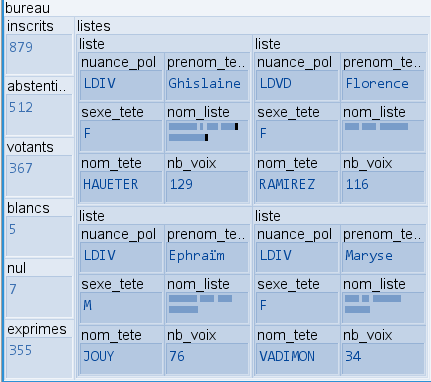
\includegraphics[width=.6\linewidth]{./src_img/contenubureau.png}
     \caption{TreeMap d'un bureau}\label{Fig:treemapbureau}
   \end{minipage}\hfill
   \begin{minipage}{0.48\textwidth}
     \centering
     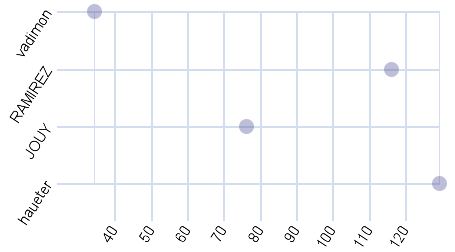
\includegraphics[width=.7\linewidth]{./src_img/graphbureau.png}
     \caption{Graphique du même bureau}\label{Fig:graphebureau}
   \end{minipage}
\end{figure}
\paragraph{}La critique qui peut être faite à BaseX est la limitation qu'elle possède au niveau des graphiques. Elle peut afficher les correspondances de plusieurs données liées aux différents objets mais ne peut traiter de requêtes. Il est donc intéressant de voir les autres possibilités.

\subsubsection{Les possibilités fournies par les outils gérant des documents}
\paragraph{}Pour le traitement de données géographiques, il peut être intéressant de réaliser des visualisations sous forme de cartes. Cependant, le jeu de données utilisé ne comprend pas les caractéristiques permettant d'en réaliser. En effet, pour avoir une représentation géographique, il est nécessaire d'avoir les coordonnées, c'est-à-dire la latitude et la longitude. Si ces données étaient présentes, des formats tels que le \acrfull{GML} ou le \acrfull{KML} auraient pu être utilisés pour afficher les informations par exemple sur Google Earth avec les données sous format \acrshort{KML}.

\paragraph{}Ces dernières années, le \newacronym{JSON}{JSON}{JavaScript Object Notation}\acrshort{JSON} est devenu de plus en plus utilisé, devenant donc une référence dans le traitement de données. Bien que moins sécurisé et non produit par l'\acrshort{OGC}, il se révèle plus léger et plus lisible que le XML \cite{xmljsoncomparison}. De nombreux outils tels que MongoDB sont familiers avec ce langage. Son dérivé, le GeoJSON s'est imposé dans le traitement de données géographiques \cite{geojsonxml}. Avec sa base venant du JavaScript, il permet une adaptation simple avec les nombreuses librairies de visualisation de données déjà présentées, Leaflet2 utilisée notamment par OpenStreetMap mais également D3.js.


\chapter{Synthèse et discussion}

\paragraph{}Ma proposition a été de comparer deux bases de données, une relationnelle, une NoSQL, sur leurs aspects techniques et leurs performances. Parti d'une même source, j'ai souhaité vérifier que la comparaison donnait l'avantage aux bases de données NoSQL. Pour ce faire, un retour sur chaque étape sera fait.

\paragraph{}Tout d'abord, la modélisation côté relationnel possède certains avantages. En effet, un formalisme, assez simple d'apprentissage, via Merise et le \newacronym{MCD}{MCD}{modèle conceptuel de données} \acrfull{MCD}, permet d'organiser les données de façon optimale. Nous ne retrouvons pas cette méthodologie côté document. Par ailleurs, la réflexion est plus importante côté relationnel afin de gérer les contraintes. De ce fait, j'attribue comme note au relationnel un 7/10 et un 5 au modèle document.

%Tout d'abord, vis-à-vis de la modélisation, le relationnel possède certains avantages. Il possède un formalisme, assez simple d'apprentissage qui permet de modéliser les données. Un \newacronym{MCD}{MCD}{modèle conceptuel de données} \acrfull{MCD} permet de préparer de manière optimale la base de données. A l'inverse, aucun formalisme est présent et commun aux modèles NoSQL, la modélisation est donc rendue plus compliquée et comme il est visible dans la figure \ref{fig:model_doc}, elle nécessite l'affichage des données. Cependant, vis-à-vis des données présentes dans le jeu initiale, la réflexion a été plus importante pour le modèle relationnel avec les contraintes à gérer. Si je dois attribuer une note, la modélisation relationnelle obtient un 7/10 et celle document un 5.

%\paragraph{}La deuxième étape est l'implémentation, elle comprend à la fois la réalisation de la structure physique et l'ajout des données. Les procédures ont été assez similaires pour le remplissage des départements, villes et bureaux avec une vérification de la présence ou non à chaque itération des données. Par la suite, l'ajout des listes et de leurs résultats a nécessité plus de vérifications côté relationnel. Cela au fait que le modèle document a uniquement besoin de reporter les données au bon endroit alors que le traitement côté relationnel doit vérifier la cohérence vis-à-vis des listes et du bureau. De ce fait, j'attribue un 6 côté document et un 4 côté relationnel.

\paragraph{}La deuxième étape est l'implémentation qui se divise en deux étapes : la création de la structure qui se réalise assez simplement des deux côtés et l'ajout des données qui possède quelques spécificités. Pour les départements, villes et bureaux de vote, le processus est assez simple. J'attribue un 4 au modèle relationnel dû aux vérifications supplémentaires nécessaires pour ajouter candidats et résultats. Ne nécessitant pas cette étape, le modèle document obtient un 7.


%C'est à l'ajout des listes ou candidats et de leurs résultats que cela diffère. En effet, côté document, les données ont uniquement besoin d'être reportées au bon endroit et les champs vides n'ont pas à être créés, c'est le cas par exemple du nom de liste, absent chez les candidats seuls. Du côté relationnel, il est nécessaire de vérifier la cohérence, de vérifier si la liste est déjà créée ou non pour éviter les erreurs à l'ajout. Egalement, le champ concernant le nom de liste peut se retrouver vide. 

\paragraph{}Pour l'interrogation, au vu de ce qui a été obtenu, il s'avèrent que les deux modèles obtiennent des résultats tout à fait convenables avec des traitements durant moins d'une seconde. Cependant, il est possible de voir que le relationnel a répondu aux requêtes un peu plus rapidement. Cela peut s'expliquer par le fait que le jeu de données utilisé soit d'une taille raisonnable pour des contraintes techniques, limitée dans notre cas aux communes d'Ile-de-France.  J'attribue donc un 6 au relationnel et un 5 au document.

\paragraph{}Concernant le dernier point, la visualisation, l'avantage de l'outil utilisé pour le modèle document, BaseX, intègre déjà des graphiques, ce qui n'est pas présent chez MySQL. Toutefois, les possibilités sont assez limités, il est donc conseillé d'utiliser des outils externes. De ce fait, j'attribue un 5 au document et un 3 au modèle relationnel dû à l'absence et les limites d'outils internes.

\paragraph{}Pour faire une synthèse de l'application, le modèle relationnel obtient une note moyenne de 5 et le document de 5,5 (figure \ref{fig:note}). On aurait pu s'attendre à de meilleures performances du NoSQL par rapport au relationnel mais comme indiqué deux paragraphes ci-dessus, les résultats obtenus sont liés au jeu de données assez limité dû aux contraintes techniques. Ce jeu étant assez léger, le relationnel arrive facilement à faire des traitements, ce qui n'aurait pas été le cas avec de plus gros jeux. L'évolution possible serait d'envisager à l'avenir d'utiliser une source de données bien plus conséquente, avec par exemple tous les résultats français, pouvant donc donner tout autre résultat. Cela pourrait être complété d'un jeu de données comprenant les caractéristiques géographiques des communes et bureaux (limites et coordonnées) afin d'avoir un rendu sous forme de carte.

\begin{figure}[!htp]
  \centering
  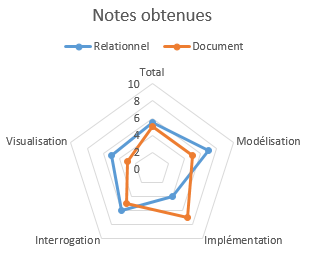
\includegraphics[width=0.5\textwidth]{./src_img/notes.png}
  \caption{Notes obtenues}
  \label{fig:note}
\end{figure}

\paragraph{}Cependant, ce que j'ai pu retenir par rapport au jeu de données choisis, c'est que l'ensemble était riche, bien structuré bien qu'avec quelques colonnes superflus car calculées, mais surtout que les données étaient figées. Dans le contexte actuel, chargé, nombre de sujets auraient pu être choisis dans le cadre de ce mémoire, comme les déplacements de population juste avant ou au début du confinement mais également l'évolution de l'épidémie de COVID-19 sur différentes échelles (locale, nationale, mondiale). Cependant, ces données s'avèrent trop changeantes, elles évoluent tous les jours, et contiennent également des erreurs.


%Je viens de voir les ajouts. Le mémoire maintenant est un peu plus riches, sauf que tu ne mets pas assez en valeur la partie application (en terme de rédaction). Je vais relire le tout en détail et te faire des suggestions.
%Sinon, le paragraphe "Évaluation de mon apport" est à développer. Personnellement j'aurais changé le titre avec "Synthèse et discussion" et enrichir la discussion. Tu expliques que tu as essayé de comparer les deux outils par rapport à 4 points: conception, implémentation, interrogation et visualisation. Ensuite, tu décris pour chaque point ton retour (il faut que ça soit personnalisé) et tu peux même donner une note (seulement par rapport à cette application). Tu peux en finir avec une figure (par exemple figure type radar) pour représenter tes notes.






%\paragraph{}Dans ma proposition, j'ai fait le choix de comparer les deux catégories de bases de données, relationnels et NoSQL, selon des critères liées aux performances. Cela correspond à quelques critères parmi l'infinité de critères possibles. 
%\paragraph{}Afin de mener cette comparaison à bien, je me suis basé sur une source de données commune. L'actualité chargée a permis de générer nombre de jeux de données potentiels : évolution de l'épidémie de COVID-19 à l'échelle locale, nationale ou mondiale, les statistiques liées au confinement telles que les déplacements de population au début de la période, les résultats d'élections. J'ai fait le choix parmi toutes ces possibilités de prendre les résultats du 1\ier tour des élections municipales de mars 2020, les autres jeux de données bougeant constamment et contenant parfois des erreurs. Vis-à-vis du jeu choisi, la totalité des données nécessaires étaient présentes mais d'autres étaient superflues car calculées à partir d'autres.



%début d'année avec corona et élections
%modification des données = plus de complexité
%adapté en fonction de mes ressources et bien sûr avec des ressources adaptées

%implémentation permet de voir les avantages du nosql mais également ces limites avec un si petit ensemble

%améliorations : quantité, structure, etc
%open data : amélioration de la sélection des données et vérification
